\section{Implementation}

\subsection{System Startup and Resource Allocation}
The entry point of the application is intentionally lightweight. In
\texttt{main.cpp}, the \texttt{setup()} function performs four steps:
\begin{enumerate}
  \item initialize the serial port and I\textsuperscript{2}C bus,
  \item allocate the application context,
  \item create queues, mutexes, and the Internet-ready semaphore, and
  \item spawn all RTOS tasks.
\end{enumerate}

This startup strategy is important because it keeps initialization
deterministic. The \texttt{loop()} function does not perform application logic;
it simply yields with a long delay. In other words, after boot the entire
system behavior is task-driven. This is a clear and appropriate RTOS pattern
for the given assignment.

The application context is initialized by \texttt{init\_app\_shared\_state()},
which sets default values such as invalid sensor readings, disconnected Wi-Fi
state, and the default LCD content mode. This avoids undefined startup
behavior.

\subsection{Shared State Helpers}
The file \texttt{global.cpp} implements helper functions to read and update the
compact shared state block. The core logic is simple but useful:
\begin{itemize}
  \item \texttt{lockSharedState()} and \texttt{unlockSharedState()} hide mutex
  handling details,
  \item \texttt{app\_set\_latest\_sensor()} updates the latest temperature and
  humidity,
  \item \texttt{app\_set\_wifi\_connected()} and
  \texttt{app\_get\_wifi\_connected()} manage connectivity state, and
  \item \texttt{app\_set\_lcd\_content\_mode()} and
  \texttt{app\_get\_lcd\_content\_mode()} coordinate LCD display policy.
\end{itemize}

The value of this module is not its complexity but its role in improving code
quality. It makes synchronization explicit and reduces the need for broad
\texttt{extern} globals. This is a meaningful improvement over directly
exposing mutable state to every file.

\subsection{Sensor Task}
The sensor task is the timing anchor of the whole application. It performs
periodic DHT20 acquisition every 2 seconds using \texttt{vTaskDelayUntil()}.
This API is a good design choice because it maintains a stable period relative
to the previous wake time, instead of accumulating drift through repeated
\texttt{delay()} calls.

The execution flow is as follows:
\begin{enumerate}
  \item initialize the DHT20 once, under I\textsuperscript{2}C mutex
  protection;
  \item on each period, attempt to lock the I\textsuperscript{2}C bus for up to
  300 ms;
  \item read temperature and humidity;
  \item if the data are valid, update the shared state and dispatch the sample
  to all consumers;
  \item if the data are invalid, propagate an invalid sample to the LCD and web
  server for graceful failure handling.
\end{enumerate}

One of the most elegant aspects of this task is the fan-out pattern. A single
physical read is turned into multiple queue writes:
\texttt{lcdQueue}, \texttt{webQueue}, \texttt{coreQueue}, and
\texttt{tinyMLQueue}. This means the sensor is sampled exactly once per period,
while the rest of the system remains modular.

\subsection{LED Manager Task}
The discrete LED task is implemented as an event-driven state machine. It does
not read sensors directly. Instead, it receives \texttt{led\_command\_t}
messages through \texttt{ledQueue}. The LED task supports two categories of
behavior:
\begin{itemize}
  \item continuous blinking according to the current temperature mode, and
  \item short pulse sequences for exceptional events.
\end{itemize}

The temperature-to-blink mapping is implemented through
\texttt{classify\_temperature\_mode()} and \texttt{led\_half\_period\_ticks()}:
\begin{itemize}
  \item cold: 5-second half-period,
  \item normal: 1-second half-period,
  \item hot: 100-ms half-period,
  \item error: 120-ms half-period.
\end{itemize}

The task also supports quick pulse bursts:
\begin{itemize}
  \item Wi-Fi connected: 3 fast blinks,
  \item error on: 6 fast blinks,
  \item error clear: stop pulsing and return to off.
\end{itemize}

The strong point of this design is that the LED module is both periodic and
reactive. It uses queue timeouts as implicit timing intervals, so it can either
wait for a new command or toggle according to the current mode without another
timer task.

\subsection{NeoPixel Task}
The NeoPixel task is simpler but still well designed. It blocks on
\texttt{neoQueue} and updates the RGB LED whenever a new humidity command
arrives. The function \texttt{humidity\_to\_color()} maps humidity into a
continuous gradient:
\begin{itemize}
  \item \(0\%\) to \(50\%\): red to green,
  \item \(51\%\) to \(100\%\): green to blue.
\end{itemize}

This is an improvement over a strict three-bin implementation because it
provides richer visual information while still satisfying the assignment's
three-level requirement. The task also supports a disable command that clears
the LED immediately, which is useful for future extension or power-saving
scenarios.

\subsection{LCD Task}
The LCD task owns the local user interface. It maintains the most recent sensor
sample and the most recent TinyML result, then decides what to show based on
system state. The logic has three levels:
\begin{enumerate}
  \item in AP mode, always show the sensor screen;
  \item in STA mode with normal LCD content mode, show the sensor screen;
  \item in STA mode with forecast LCD content mode, show the TinyML forecast.
\end{enumerate}

This conditional behavior is an excellent example of policy separation. The
task itself decides \textit{how} to render each screen, while the rest of the
system decides \textit{which content mode} is currently active.

The LCD module also reacts to environmental context:
\begin{itemize}
  \item if the sensor data are invalid, it prints \texttt{Sensor Error};
  \item if Wi-Fi is connected, it can display signal quality in percent and a
  qualitative label such as \texttt{GOOD} or \texttt{WEAK};
  \item if TinyML results exist, it shows forecast label and rain probability.
\end{itemize}

An important implementation detail is that LCD rendering is not performed at a
fixed blind period. Instead, the task updates when a new sensor sample arrives,
when TinyML changes, when RSSI changes meaningfully, or when AP/STA mode
changes. This avoids unnecessary I\textsuperscript{2}C traffic and makes the
display more event-aware.

\subsection{Web Server Task}
The web module is the largest subsystem in the repository. It combines
\texttt{WebServer}, \texttt{Preferences}, local runtime state, and Wi-Fi mode
management. Its implementation can be divided into five functional groups.

\subsubsection*{1) AP/STA workflow.}
The board starts either from the most recently saved Wi-Fi profile or directly
in AP mode if no profile exists. The helper functions
\texttt{startApMode()} and \texttt{startStaConnect()} reset Wi-Fi state,
configure the correct mode, and update internal status flags. If STA connection
fails after 10 seconds, the system automatically returns to AP mode. The BOOT
button also forces AP mode manually.

\subsubsection*{2) Persistent Wi-Fi profiles.}
The project uses \texttt{Preferences} to store up to five Wi-Fi profiles. The
most recently used profile is kept at index 0. The code supports:
\begin{itemize}
  \item reading saved profiles,
  \item updating or inserting a profile,
  \item removing all saved profiles.
\end{itemize}
This is a practical improvement because it lets the board remember STA
credentials across restarts without hard-coding a single network.

\subsubsection*{3) AP dashboard and settings pages.}
The root page in AP mode displays:
\begin{itemize}
  \item temperature and humidity,
  \item TinyML label and probability,
  \item AP IP and Wi-Fi status,
  \item target STA SSID and STA IP,
  \item external LED control,
  \item chart history, and
  \item quick Wi-Fi scan results.
\end{itemize}
The settings page expands the Wi-Fi management workflow by providing scan,
saved-profile, and connect forms. The STA page is intentionally simpler and
acts mainly as a status page rather than a full dashboard.

\subsubsection*{4) REST endpoints.}
The task registers multiple routes:
\begin{itemize}
  \item \texttt{/} for the main page,
  \item \texttt{/settings} for Wi-Fi configuration,
  \item \texttt{/api/state} for live JSON state,
  \item \texttt{/api/scan} for Wi-Fi scan results,
  \item \texttt{/api/saved} for stored Wi-Fi profiles,
  \item \texttt{/connect} for STA connection request,
  \item \texttt{/forget} for profile reset,
  \item \texttt{/api/light/toggle} for on/off control,
  \item \texttt{/api/light/brightness} for PWM brightness control.
\end{itemize}

\subsubsection*{5) STA Mode (Cloud Integration and Remote Configuration)}
When the device successfully establishes a connection to a Wi-Fi network, the Web Server transitions to a specialized configuration portal. This interface is crucial for defining where and how the system's telemetry data is routed:
\begin{itemize}
    \item \textbf{Dynamic Broker Configuration:} The STA page provides a dedicated form for customizing the communication target. Users can input the \textbf{MQTT Broker Host (Server Name)}, \textbf{Username}, and \textbf{Password} directly through the browser. This allows the system to be pointed to the official CoreIOT platform, a private MQTT broker, or a custom **Local Server** without any code changes.
    \item \textbf{Persistence and REST API:} Configuration changes are submitted via the \texttt{/api/coreiot/config} POST endpoint. The task processes these requests and uses the \texttt{Preferences} library to save the credentials into the \texttt{WIFI\_STORE\_NAMESPACE}, ensuring the settings persist even after a power cycle.
    \item \textbf{CoreIOT Task Synchronization:} The \texttt{coreiot\_task} is designed to be reactive to these changes. When a new server host or set of credentials is saved, the web task updates the shared application context. The CoreIOT task, which is constantly monitoring the connection state, will automatically trigger a reconnection sequence to the newly specified server.
    \item \textbf{Telemetry Routing Control:} The interface also includes a toggle to enable or disable publishing. This gives the user full control over data privacy, allowing them to stop cloud transmission or redirect the stream to a local endpoint for private data logging.
\end{itemize}

\begin{figure}[H]
    \centering
    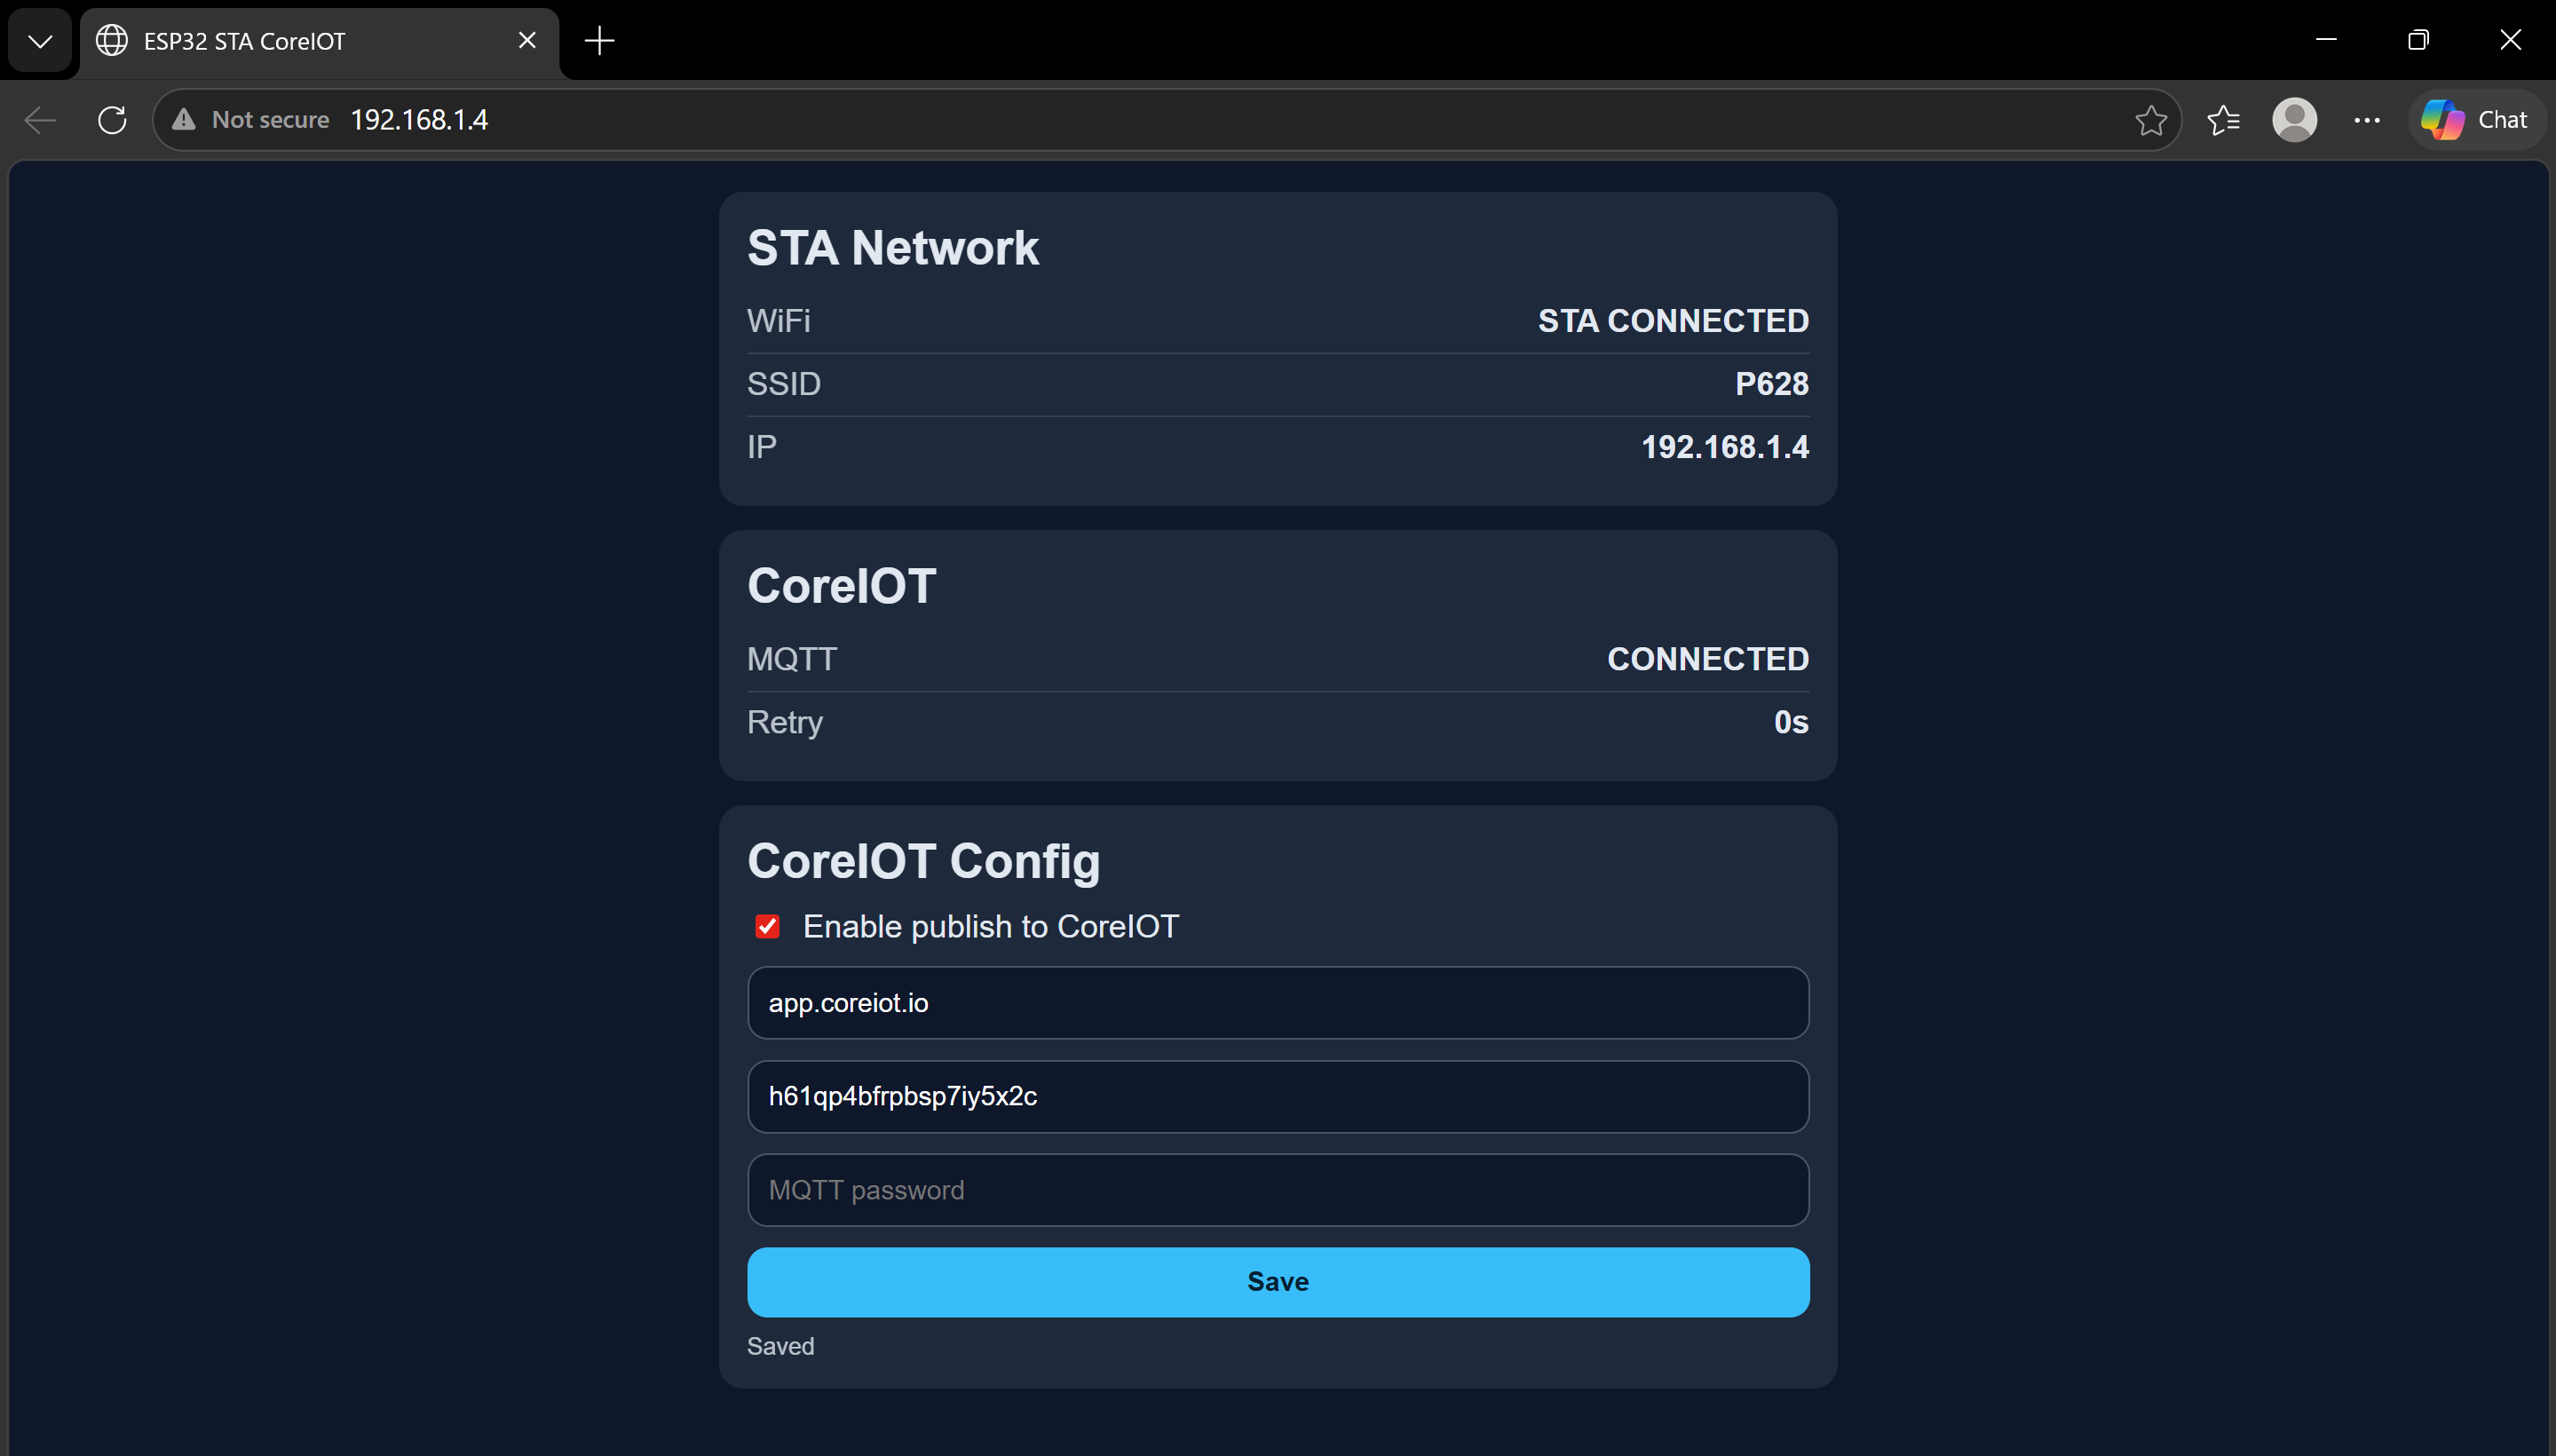
\includegraphics[width=1\textwidth]{images/f1.png} 
    \caption{Webserver STA UI}
\end{figure}

\subsubsection*{6) Client-side visualization.}
The AP dashboard includes JavaScript that polls \texttt{/api/state} every 2
seconds. It updates visible values and renders a chart on a
\texttt{canvas}. A recent improvement in the code is the use of dual Y-axes for
temperature and humidity, which avoids the misleading effect of drawing both
series on a single implicit scale. The chart also displays axis labels and
relative sample times.

Two implementation highlights stand out in this module. First, the task uses a
20 ms loop period, which is short enough for responsive HTTP handling without
busy-waiting. Second, the cloud subsystem is not started blindly; instead, the
web task signals \texttt{internetSemaphore} once STA connectivity is confirmed.


\subsection{TinyML Task: Edge-Based Rain Forecasting Pipeline}

The TinyML task implements an on-device rain prediction system, shifting the analytical workload from the cloud directly to the edge. This approach minimizes latency, reduces network dependency, and demonstrates the viability of executing neural networks on resource-constrained microcontrollers. The development and deployment of this predictive model follow a comprehensive Machine Learning pipeline, spanning from offline dataset preparation to real-time RTOS integration.

\subsubsection*{1) Dataset Overview and Preprocessing}
The predictive model is built upon a historical meteorological dataset collected in Ho Chi Minh City, encompassing continuous weather observations from 2009 to 2020. The primary objective is to perform a binary classification, categorizing the upcoming weather state as either "RAIN" (Class 1) or "SUNNY/SAFE" (Class 0). 

During the offline data preparation phase, the raw weather labels were grouped to form the binary target variable. Conditions containing keywords such as 'rain', 'thunder', 'drizzle', or 'storm' were mapped to Class 1, while all other conditions were mapped to Class 0. To ensure the neural network converges effectively during training, the input features were standardized using \texttt{StandardScaler}, giving the data a mean of zero and a variance of one.

\subsubsection*{2) Feature Engineering and Extraction}
The edge system relies on a single DHT20 sensor to capture ambient temperature and humidity. To maximize the predictive power of this single data source, the system does not feed raw, instantaneous readings directly into the model. Instead, it derives an 8-feature input vector designed to capture both environmental trends and cyclical temporal patterns:
\begin{enumerate}
    \item \textbf{Batch Averages ($T_{avg}, H_{avg}$):} The mean temperature and humidity are calculated over a sliding window. Filtering out momentary sensor noise provides a stable baseline of the current microclimate.
    \item \textbf{Temporal Deltas ($\Delta T, \Delta H$):} The difference between the current batch averages and the previous batch averages. This captures the dynamic rate of change (e.g., a sudden drop in temperature combined with rapidly rising humidity), which is a critical meteorological indicator for incoming rain.
    \item \textbf{Cyclical Time Features ($\sin(m), \cos(m), \sin(h), \cos(h)$):} Time is inherently cyclical, but standard integer representations (e.g., hour 23 and hour 0) appear mathematically distant to a neural network. By transforming the current month and hour using sine and cosine functions, the model correctly interprets the continuous, circular nature of time, helping it recognize diurnal variations and seasonal monsoon patterns in Ho Chi Minh City.
\end{enumerate}

\subsubsection*{3) Model Architecture and Training}
The core logic is driven by a sequential Artificial Neural Network (ANN) designed via TensorFlow/Keras. The architecture is intentionally lightweight to accommodate the ESP32-S3's memory constraints while remaining capable of capturing non-linear relationships within the 8 features. The network topology consists of:
\begin{itemize}
    \item An \textbf{Input Layer} accepting the 8 standardized features.
    \item A \textbf{Hidden Dense Layer} with 12 neurons utilizing the ReLU (Rectified Linear Unit) activation function.
    \item A \textbf{Second Hidden Dense Layer} with 8 neurons, also using ReLU activation.
    \item An \textbf{Output Layer} with a single neuron applying a Sigmoid activation function, producing a final probability score between 0.0 and 1.0.
\end{itemize}

During the offline training phase, the dataset was split into an 80\% training set and a 20\% testing set. The model was compiled using the Adam optimizer and a binary cross-entropy loss function. After training for 50 epochs with a batch size of 32, the baseline model achieved an impressive accuracy of \textbf{84.45\%} on the 32-bit floating-point (float32) test set.

\subsubsection*{4) Full Integer Quantization for Edge Deployment}
To deploy this trained model onto the ESP32-S3, it required an aggressive optimization process using the TensorFlow Lite Converter. Deploying a float32 model would consume excessive SRAM and execution time. Therefore, the model underwent \textbf{Full Integer Quantization (INT8)}.

A Representative Dataset generator (yielding 100 random training samples) was used to calibrate the dynamic range of the model's weights and activations. This calibration allowed the converter to safely map the 32-bit floats into 8-bit integers. The resulting optimized model (\texttt{.tflite}) was then converted into a C-byte array header file (\texttt{model\_data.h}) using the \texttt{xxd} utility. 

Remarkably, after this strict quantization process, the model retained an accuracy of approximately \textbf{83\%}. This minor degradation (around 1.45\%) is a highly favorable trade-off, as the INT8 model drastically reduces the memory footprint and accelerates inference time on the microcontroller without utilizing floating-point hardware during the forward pass.

\subsubsection*{5) C++ Implementation in the RTOS Environment}
Within the firmware, the \texttt{tiny\_ml\_task} manages the real-time execution of this pipeline. It utilizes the \texttt{tflite::MicroInterpreter} and an \texttt{AllOpsResolver} initialized with a 16 KB tensor arena. The implementation strictly mirrors the offline training pipeline:
\begin{itemize}
    \item \textbf{Accumulation:} The task receives raw data from \texttt{tinyMLQueue} and accumulates 10 consecutive sensor samples (equivalent to a 20-second monitoring window) before triggering an inference cycle.
    \item \textbf{Normalization:} The computed 8 features are standardized locally using pre-computed \texttt{means} and \texttt{scales} arrays extracted from the Python \texttt{StandardScaler}.
    \item \textbf{Input Quantization:} The normalized float values are converted into the INT8 format required by the model using the input tensor's specific \texttt{scale} and \texttt{zero\_point} parameters.
    \item \textbf{Inference and Output:} The \texttt{interpreter->Invoke()} function is called. The resulting INT8 output is de-quantized back into a float probability. If this probability exceeds the 0.5 threshold, the system categorizes the upcoming state as "RAIN".
\end{itemize}

Finally, this prediction, along with the calculated probability percentage and timestamps, is packaged into a \texttt{tinyml\_result\_t} structure and pushed to the \texttt{tinyResultQueue}. It is subsequently consumed by the LCD task for immediate local display and by the CoreIOT task for remote cloud telemetry.
\subsection{CoreIOT Task}
The CoreIOT task is responsible for MQTT connectivity and telemetry publishing.
Its logic is intentionally staged and highly configurable:
\begin{enumerate}
  \item wait on \texttt{internetSemaphore},
  \item retrieve dynamic MQTT connection parameters (broker host/IP, username, password) configured via the web interface,
  \item connect to the specified MQTT broker,
  \item subscribe to the RPC request topic,
  \item periodically publish telemetry every 10 seconds.
\end{enumerate}

A significant architectural extension in this module is its support for dynamic server integration. The MQTT broker host and credentials are not strictly hard-coded into the firmware. Instead, the task retrieves these settings from the persistent configuration managed by the Web Server task. This allows users to easily redirect the telemetry stream from the default CoreIOT cloud platform to a custom local MQTT broker by simply updating the host IP address via the STA web interface. This extensibility ensures the system can seamlessly adapt to private, local IoT deployments on the fly, entirely without the need to modify source code or recompile the firmware.

The telemetry payload includes:
\begin{itemize}
  \item temperature,
  \item humidity,
  \item timestamp (epoch if valid, otherwise tick-based fallback),
  \item rain probability,
  \item rain probability percentage,
  \item categorical rain prediction,
  \item short rain status string,
  \item current LCD forecast mode,
  \item Wi-Fi connection state.
\end{itemize}

This payload is a good design choice because it combines raw measurements with
derived context. The cloud dashboard therefore has richer observability than a
minimal two-field sensor upload.

The CoreIOT task also supports remote control through RPC. It accepts several
method aliases, parses flexible boolean-like parameters, and maps the result to
LCD content mode. In practice, this means a cloud-side control widget can switch
the local LCD between sensor display and TinyML forecast display during STA
operation.

\subsection{Time Utility Module}
The file \texttt{app\_time\_utils.cpp} provides helper routines for:
\begin{itemize}
  \item validating epoch time,
  \item converting epoch time into local date-time fields,
  \item synchronizing with NTP, and
  \item formatting time strings.
\end{itemize}

Although the current runtime path does not actively show a complete NTP setup
sequence, this module is still important because both the TinyML and CoreIOT
parts are time-aware. It creates a clean extension point for future work in
which telemetry timestamps and time-derived inference features are backed by
live synchronized clock values.

\begin{figure}[H]
    \centering
    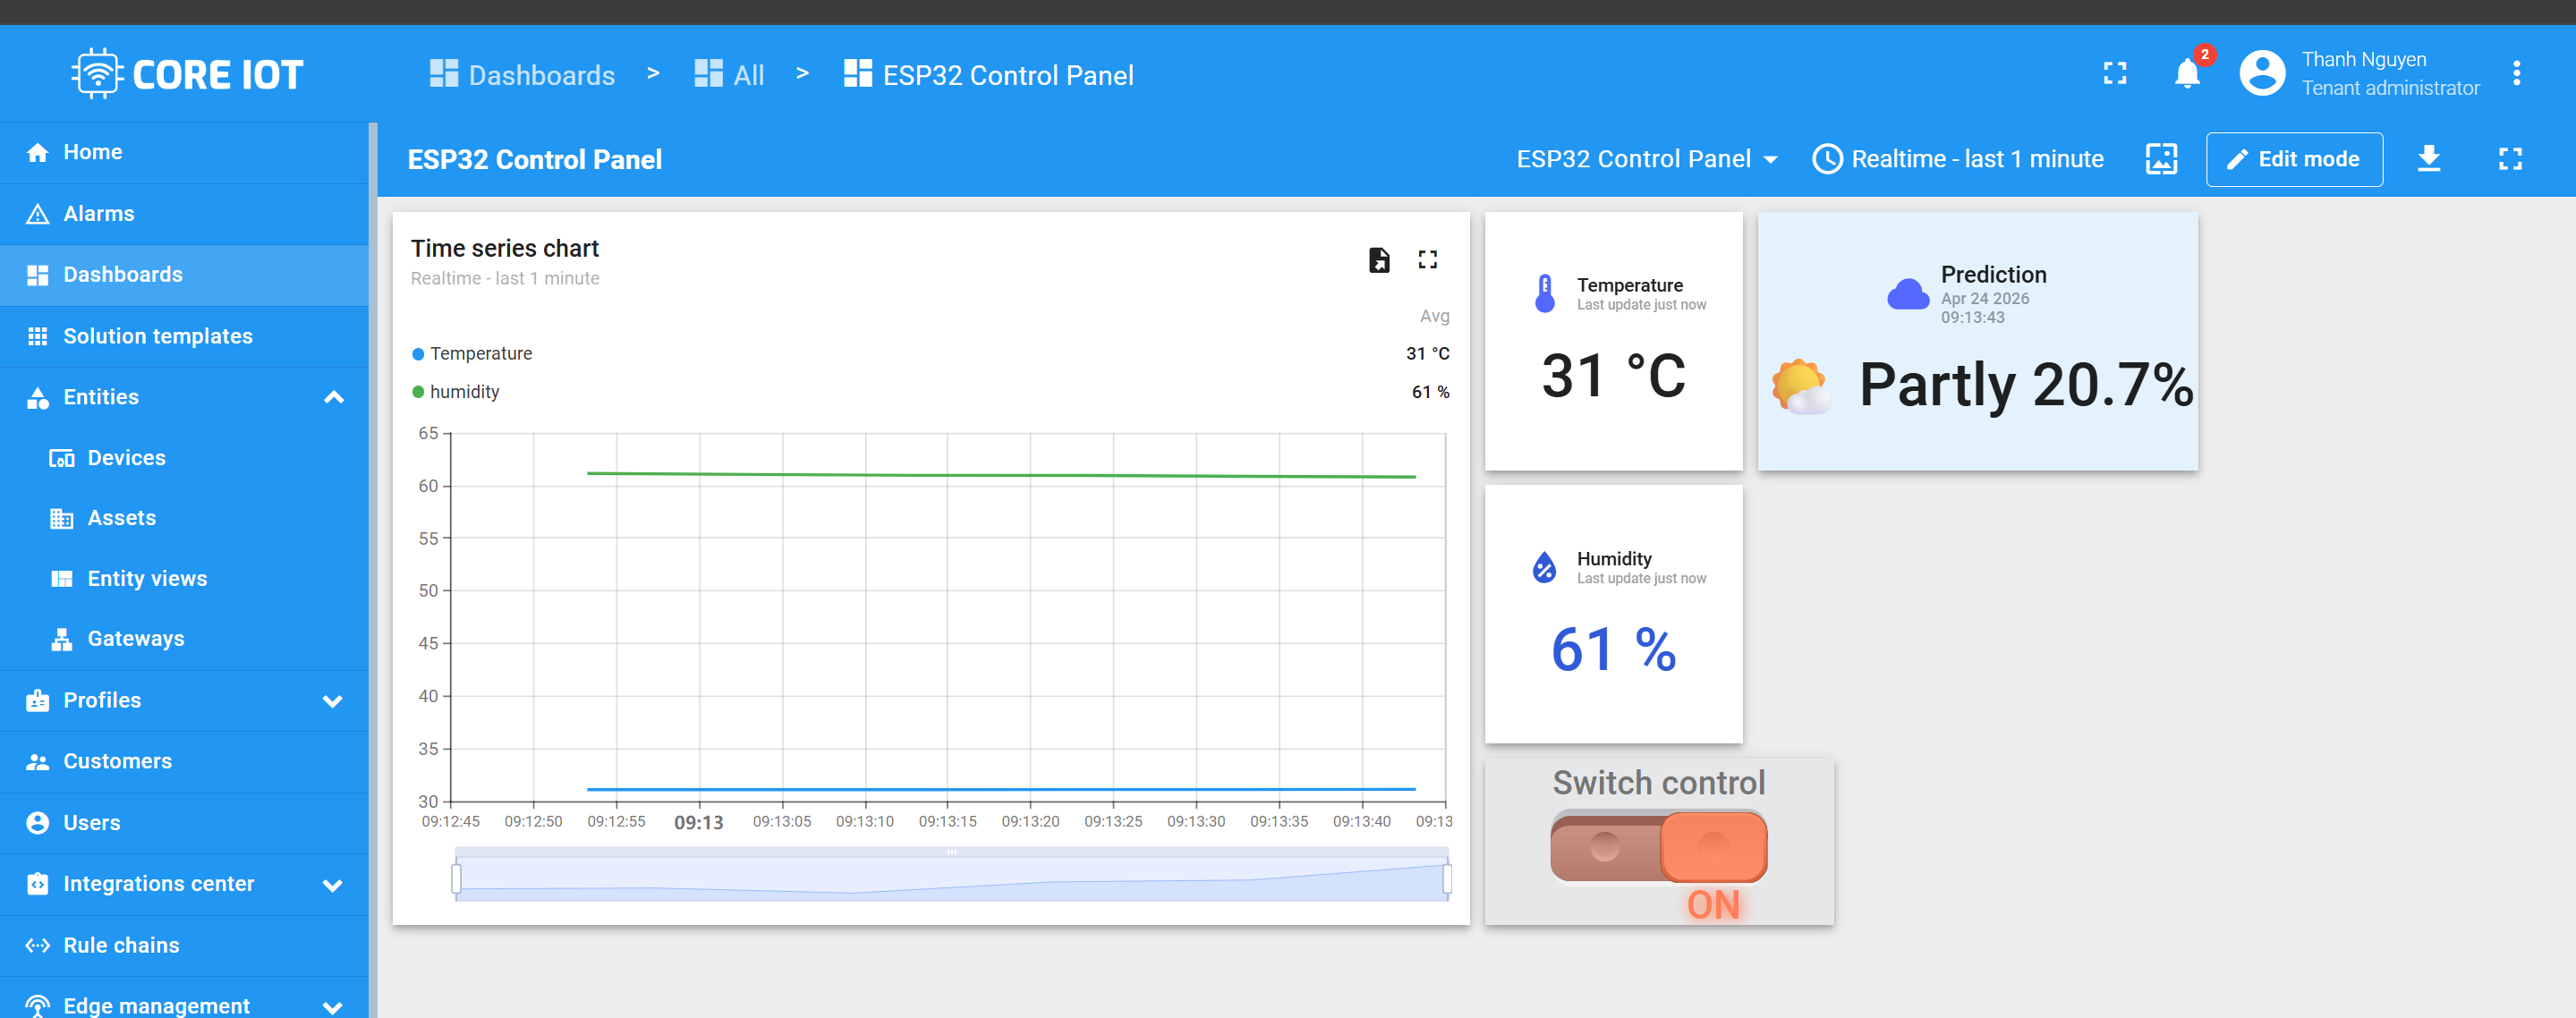
\includegraphics[width=1\textwidth]{images/f2.png} 
    \caption{coreIOT dashboard}
\end{figure}


\subsection{Implementation Qualities}
Several implementation features are worth highlighting as strengths of the
project:
\begin{itemize}
  \item The system uses \texttt{xQueueOverwrite()} effectively for latest-value
  semantics.
  \item The sensing period is stabilized through \texttt{vTaskDelayUntil()}.
  \item Shared state is reduced and protected by a mutex.
  \item The LCD behavior is policy-driven rather than hard-coded to one screen.
  \item The web interface is not a static page; it actively supports monitoring,
  configuration, and control.
  \item The TinyML task is integrated into the same RTOS pipeline as the other
  system functions.
  \item The CoreIOT task supports both telemetry and remote RPC interaction.
\end{itemize}

Taken together, these implementation choices show that the system is not merely
feature-complete for the assignment; it is architecturally coherent.
